\chapter{RE-TOOL}\label{chap:approach}

\section*{}

%Este capítulo deve começar por fazer uma apresentação detalhada do problema a resolver\footnote{Na introdução a apresentação do problema foi breve.} podendo mesmo, caso se justifique, constituir-se um capítulo com essa finalidade.

%Deve depois dedicar-se à apresentação da solução sem detalhes de implementação. Dependendo do trabalho, pode ser uma descrição mais teórica, mais ``arquitetural'', etc.
In this chapter, we begin by giving a brief overview of PBGT, the research project the developed work is inserted in. Afterwards, the previous approach and current tool are broken down in components and explained in detail.

\section{PBGT Overview}\label{sec:pbgt}

As mentioned before, the focus of this dissertation is the reverse engineering component of a research project named PBGT (\textit{Pattern-based GUI Testing}) \cite{moreira2013pattern}. The goal of this project is to develop a model-based GUI testing approach and supporting tool, that can be used in industrial contexts.\\

\subsection{Architecture}
The PBGT supporting tool has main five components: 
\begin{enumerate}
\item \textbf{PARADIGM}, a DSL (\textit{Domain Specific Language}) to define GUI testing models based on UI Test Patterns \cite{enase14}; 
\item \textbf{PARADIGM-RE}, a Web application reverse engineering tool whose purpose is to extract UI patterns from Web pages without access to their source code, and use that information to generate a test model written in PARADIGM; 
\item \textbf{PARADIGM-ME}, a modeling and testing environment, built to support the creation of test models \cite{conf_icst_MonteiroP13}; 
\item  \textbf{PARADIGM-TG}, an automatic test case generation tool that generates test cases from test models defined in PARADIGM according to coverage criteria selected by the tester; 
\item and finally, a test case execution tool, named \textbf{PARADIGM-TE}, which executes test cases, analyzes their coverage with a coverage analysis tool named \textbf{PARADIGM-COV}\cite{vilela2014cov}, and returns detailed execution reports. 
\end{enumerate}

The architecture and workflow of the project is shown in Fig. \ref{fig:pbgt}.\\

\begin{figure}[!htb]
\centering
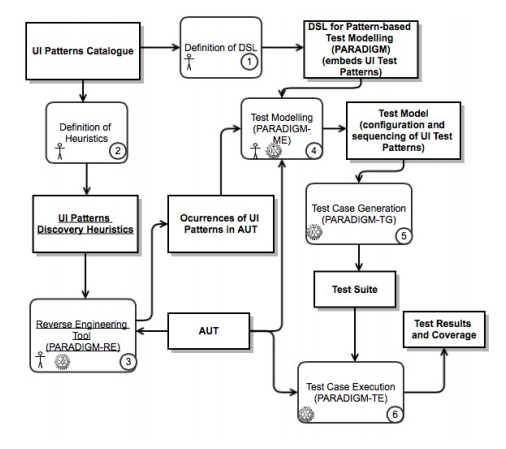
\includegraphics[width=\textwidth]{pbgt}
\caption{An overview of the PBGT project.}
\label{fig:pbgt}
\end{figure}

\subsection{PARADIGM DSL}\label{sec:dsl}
%falar doc conetores e, do init e do end, e falar também dos elementos estruturais: Form e Group

PARADIGM is a DSL to be used in the domain of PBGT. The goal of the language is to gather applicable domain abstractions (e.g., UI test patterns), allow specifying relations between them and also provide a way to structure the models in different levels of abstraction to cope with complexity. PARADIGM's meta-model is illustrated in Figure \ref{fig:dsl}.\\

\begin{figure}[!htb]
\centering
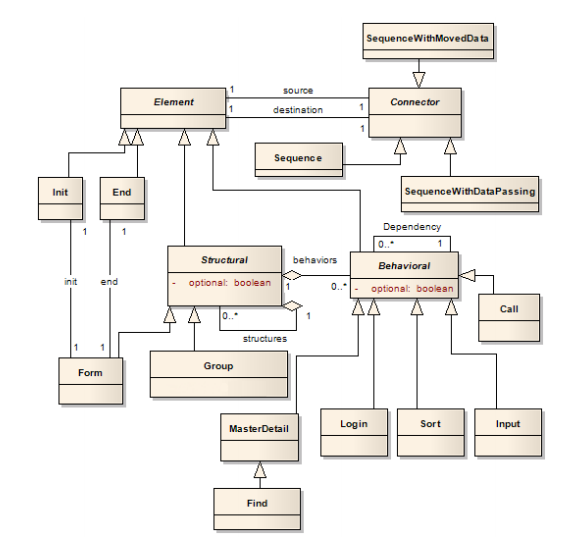
\includegraphics[width=\textwidth]{dsl}
\caption{PARADIGM DSL Meta-model.}
\label{fig:dsl}
\end{figure}

The PARADIGM language is comprised by elements and connectors \cite{moreira2013pattern}. There are four types of elements: \textit{Init} (to mark the beginning of a model), \textit{End} (to mark the termination of a model), \textit{Structural} (to structure the models in different levels of abstraction), and \textit{Behavioral} (UI Test Patterns describing the testing goals).\\

As models become larger, coping with their growing complexity forces the use of structuring techniques such as different hierarchical levels that allow use one entire model \textbf{A} inside another model \textbf{B} abstracting the details of \textbf{A} when within \textbf{B}. Structuring techniques are common in programming languages like C and Java, with constructs such as modules and classes. \textit{Form} is a structural element that may be used for that purpose. A \textit{Form} is a model (or sub-model) with an \textit{Init} and an \textit{End} elements. \textit{Group} is also a structural element but it does not have \textit{Init} and \textit{End} and, moreover, all elements inside the \textit{Group} are executed in an arbitrary order.\\

\begin{figure}[!htb]
\centering
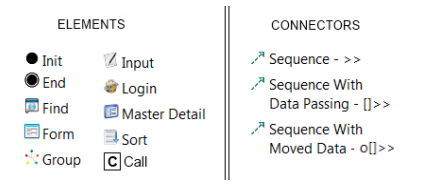
\includegraphics[width=0.5\textwidth]{dsl1}
\caption{PARADIGM syntax.}
\label{fig:dsl1}
\end{figure}

PARADIGM elements and connectors are described by: (i) an icon/figure to represent the element graphically and (ii) a short label to name the element. The overall syntax of the DSL is illustrated in Figure \ref{fig:dsl1}. Additionally, elements within a model have a number to identify them, and optional elements have a ``op" label next to its icon/figure.\\

This language has three connectors: \textit{Sequence}, \textit{SequenceWithDataPassing}, and \textit{SequenceWithMovedData}. \textit{Sequence} indicates that the testing strategy related to the target element cannot start until the testing strategy of the source element has completed. \textit{SequenceWithDataPassing} has the same meaning as \textit{Sequence}, and additionally indicates that the target element receives data from the source element. \textit{SequenceWithMovedData} has a similar meaning to \textit{SequenceWithDataPassing}, but the source element moves data to the target instead of transferring a copy. In addition, there is another kind of relation among elements -- \textit{Dependency} -- indicating that the target element depends on the properties of a set of source elements, for instance, when it is the result of a calculation. \\

\subsubsection{UITP (User Interface Test Patterns)}

A UI Test Pattern defines a test strategy to test a specific UI pattern, which is formally defined by a set of test goals (for later configuration)\cite{moreira2013pattern} with the form:

\begin{equation}< Goal; V; A; C; P >\end{equation}\label{eq:ui_}

\textit{Goal} is the \textit{ID} of the test. \textit{V} is a set of pairs { [\textit{variable}, \textit{inputData}] } relating test input data with the variables involved in the test. \textit{A} is the sequence of actions to perform during test case execution. \textit{C} is the set of possible checks to perform during test case execution, for example, “check if it remains in the same page”. \textit{P} is a Boolean expression (precondition) defining the set of states in which it is possible to execute the test. The language also defines language constraints to guarantee the building of well-formed models, such as ``\textit{A Connector cannot connect an element to itself}'' and ``\textit{A Connector cannot have Init as destination, or End as source}'', to cite a few examples.\\

The UI Patterns defined in the PARADIGM language are:
\begin{itemize}
\item \textbf{Login}: This pattern is commonly found in Web applications, especially in the ones that restrict access to functionalities or data. Usually consists of two input fields (a normal input box for email or username, and a cyphered text for the password) and a submit button, with optionally a ``remember me'' checkbox. The authentication process has two possible outcomes: valid and invalid. Upon authentication failure a message may be shown. 
\item \textbf{Find}: This pattern consists of one or more input fields, where the user inserts keywords to search, and a submit button to start the search. The search may be submitted via a submit button, or dynamically upon text insertion. When the search is successful, the website shows a list of results; upon failure, an error message may be shown.
\item \textbf{Sort}: This pattern sorts a list of data by a common attribute (e.g., price, name, relevance, etc.) according to a defined criteria (ascending or descending, alphabetically, etc.).
\item \textbf{Master Detail}: This pattern is present in a web page when selecting an element from a set (called \textit{master}) results in filtering/updating another related set (called \textit{detail}) accordingly. For example, clicking on a checkbox associated to a brand may include (or exclude) products of that brand in a product search result list. Generally the only elements changed are the elements belonging to the \textit{detail} set.
\item \textbf{Call}: This pattern is any kind of element where a click triggers some procedure that may result in a change of page.
\end{itemize}

\subsection{Produced Models}

The models produced by the reverse engineering tool PARADIGM-RE consist of a XML file in the format required by the PARADIGM-ME which contains information about the UI Test Patterns needed to test the UI Patterns found: their name, the input values for their variables, i.e., the values used during the exploration process, and blank pre-conditions and checks for the tester to fill in. The UI Test Patterns within the model are connected in a linear path according to the exploration order. The testing configuration information needs to be complemented and validated by the tester afterwards in order to generate test cases and execute them over the web application under analysis.

\section{Reverse Engineering Approach}\label{sec:re}

\subsection{Previous Tool}\label{sec:prev}

The  approach described in this dissertation aims to improve on the previous work \cite{nabuco2013inferring} done on the PARADIGM-RE tool. In particular it aims to be fully automatic. The previous tool required the intervention of the user to interact with the web application under analysis in order to save the interaction traces and proceed from there. It extracted information from an user's interaction with the Web application under analysis, analyzed the information, produced some metrics (such as the total ratio of the LOC (\textit{lines of code}), length of all visited pages and the ratio of two subsequent pages), and finally used those metrics and the user interaction's information to infer UI patterns via a set of heuristic rules. \\
This tool identifies interface patterns using Machine Learning inference with the Aleph ILP system \footnote{Aleph: \url{http://www.cs.ox.ac.uk/activities/machlearn/Aleph/aleph\_toc.html}} running on user interaction execution traces produced using Selenium \footnote{Selenium: \url{http://docs.seleniumhq.org/}}. It was deemed necessary then to transform the whole process into an iterative one, with the model being updated at every iteration. 

This was accomplished in \cite{nabuco2014inferring}, where the tool was extended with a pattern identifying module using heuristics. The structure of the previous tool can be seen in Figure \ref{fig:retool_prev}. 

\begin{figure}[!htb]
 \begin{center}
 \leavevmode
 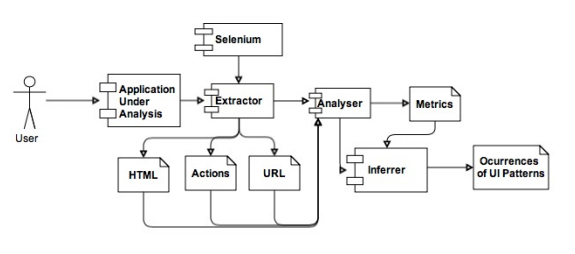
\includegraphics[width=\textwidth]{retool_prev}
 	\caption[Structure of the PARADIGM-RE tool]{Structure of the PARADIGM-RE tool \cite{nabuco2014inferring}}
 	\label{fig:retool_prev}
 \end{center}
\end{figure}

The user interacts with the Web application, using Selenium to save the actions taken. An example of execution traces saved by Selenium can be seen on table \ref{tab:amazontraces}. 

\begin{table}[!htb]
\begin{tabular}{|l|l|l|}
\hline
\multicolumn{3}{|c|}{\textbf{amazon}} \\ \hline
\textbf{actionType} & \textbf{element} & \textbf{text} \\ \hline
open & / & \\ \hline
type & id=twotabsearchtextbox & tablet \\ \hline
clickAndWait & css=input.nav-submit-input & \\ \hline
select & id=sort & label=Most Popular \\ \hline
click & id=pagnNextString & \\ \hline
click & id=pagnPrevString & \\ \hline
clickAndWait & link=Image & \\ \hline
clickAndWait & link=Detail & \\ \hline
click & link=android tablet & \\ \hline
click & css=li.refinementImage \textgreater a.. \textgreater span.refinementLink & \\ \hline
clickAndWait & css=\#result\_3 \textgreater h3.newaps \textgreater a \textgreater span.lrg.bold & \\ \hline
clickAndWait & link=Explore similar items & \\ \hline
\end{tabular}
\caption[An example of execution traces produced on the Amazon.com website, extracted using Selenium IDE.]{An example of execution traces produced on the Amazon.com website, extracted using Selenium IDE\protect\footnotemark.}
\label{tab:amazontraces}
\footnotetext{Selenium IDE: \url{http://docs.seleniumhq.org/}}
\end{table}

The \textbf{extractor} saves the HTML of all pages visited, their URLs, and the actions taken in each page. All that information is passed along to the \textbf{analyzer}, whose purpose is to produce metrics like page ratios, differences between consecutive pages, and others, from the data given. Those metrics are passed to the \textbf{inferrer}, who runs the heuristics suite, identifies existing patterns, and produces a XMI file with the occurrences found. An example of the contents of such a file, with one of each inferrable pattern, can be found on Listing \ref{lst:paradigm}.

\lstset{language=XML,caption={An example of a .paradigm file with identified patterns},label=lst:paradigm}
\begin{lstlisting}
<?xml version="1.0" encoding="UTF-8"?>
<Paradigm:Model xmi:version="2.0" xmlns:xmi="http://www.omg.org/XMI"
 xmlns:Paradigm="http://www.example.org/Paradigm" title="patterns"/>
	<nodes xsi:type="Paradigm:Init" name="XInit" number="1"/>
	<nodes xsi:type="Paradigm:Sort" name="Sort2" number="2"/>
    <nodes xsi:type="Paradigm:Login" name="Login3" number="3"/>
    <nodes xsi:type="Paradigm:MasterDetail" name="MasterDetail4" number="4"/>
    <nodes xsi:type="Paradigm:Input" name="Input5" number="5"/>
    <nodes xsi:type="Paradigm:Find" name="Find6" number="7"/>
	<nodes xsi:type="Paradigm:End" name="End" number="8"/>
</Paradigm:Model>
\end{lstlisting}

This approach was evaluated on several worldwide used Web applications and the results were deemed satisfactory, since the tool identified most of the occurring patterns and their location on the page. However, there are some patterns the tool doesn't identify, such as the Menu pattern, and the high number of false positive results indicate the heuristics are considered to be still in an incipient state.

The information saved from a user interaction was the source code and URLs of the visited pages, and the interaction's execution trace. An execution trace is the sequence of user actions executed during the interaction with a software system, such as clicks, text inputs and also some information of the system state (e.g., the information that is being displayed). An example of an execution trace file used by the tool can be seen in Table \ref{tab:exec}.\\

\begin{table}[!htb]
\resizebox{0.9\textwidth}{!}{
  \begin{tabular}{| c | c | c |}
     \hline
     \textbf{Action} & \textbf{Target} & \textbf{Value} \\ \hline
     type&id=input\_username &``user1" \\ \hline
     type&id=input\_password &``123pass" \\ \hline
     clickAndWait & css=input[type=``submit"]&EMPTY \\
     \hline
     type&id=searchInput&``coffee" \\ \hline
	 clickAndWait & id=mw-searchButton&EMPTY\\
     \hline
     select&id=sort&label=Price:Low to High \\
     \hline
     %%%%%
     click&id=collapseButton1&EMPTY\\\hline
     click&link=Next&EMPTY\\\hline
     typeAndWait&id=freeSearch&ministry\\\hline
     type&id=authcode&T75Y5\\\hline
     type&name=firstName&james\\\hline
	 type&name=lastName&bond\\\hline
     click&//ul[@id='ref1']/li[5]/a/span&EMPTY\\\hline
  	 \end{tabular}
}
\caption{Abbreviated example of an execution trace file.}
\label{tab:exec}
\end{table}

The previous reverse engineering approach identified the \textit{Find}, \textit{Login}, \textit{Sort}, \textit{Input} and \textit{MasterDetail} patterns, and produced a high number of false positives \cite{nabuco2013inferring}. Additionally, and as already mentioned, the exploration process was done by saving the user interaction with the Web application under test, requiring human interaction to identify patterns. The results were dependent on the execution traces followed by the tester. \\

\subsection{Current Tool}

The work described in this dissertation is a completely new tool, unrelated to the previous tool, but which has the same primary aim as the previous tool (to identify UI patterns in the Application Under Test (AUT)), only with other goals. The first is to remove the need for user interaction with the AUT to identify patterns, by providing a reverse engineering process to explore automatically the web application under analysis. The second is to refine and improve the pattern inferring process, and lower or eliminate completely the percentage of false positives. The third is to identify more patterns than the previous tool (including patterns that are going to be included in latter versions of the PARADIGM DSL, like the Menu pattern).\\

The architecture of the tool is seen in Figure \ref{fig:retool}.
\begin{figure}[!htb]
\centering
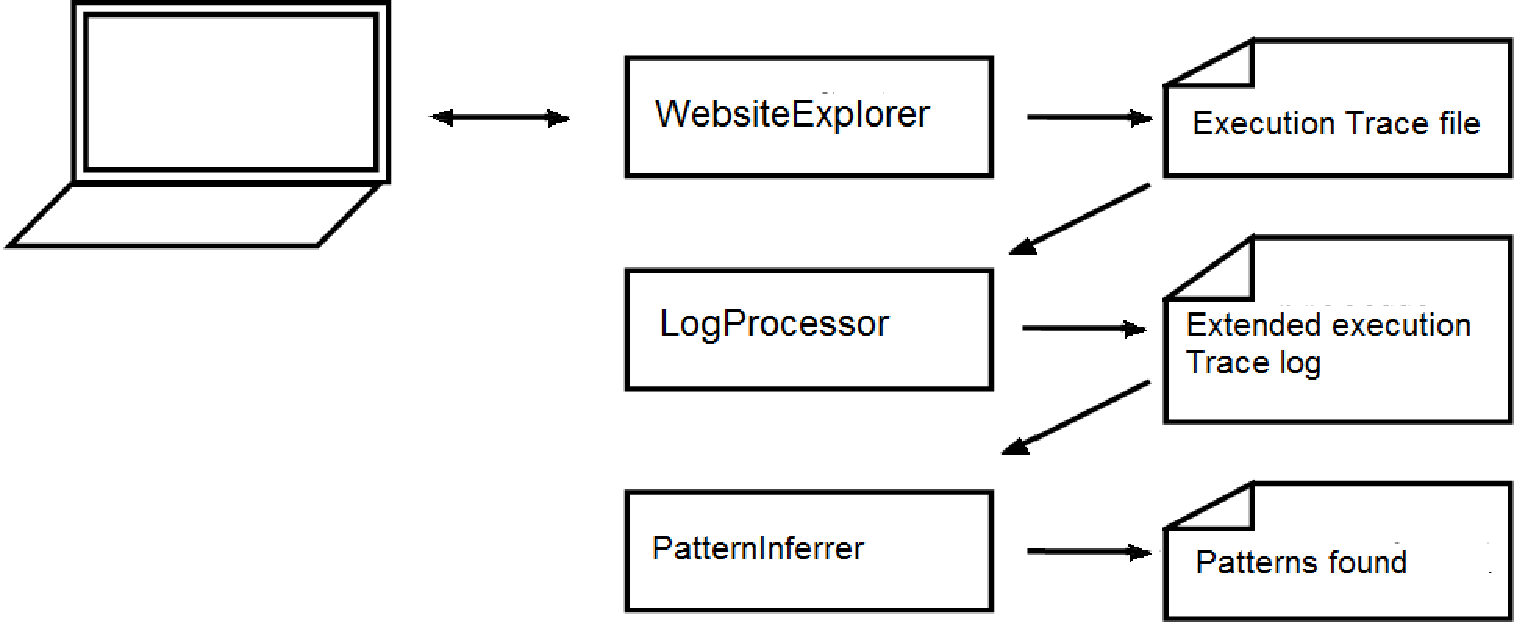
\includegraphics[width=\textwidth]{retool}
\caption{The architecture of the approach.}
\label{fig:retool}
\end{figure}

The approach can be divided into three parts: \textbf{WebsiteExplorer}, \textbf{LogProcessor}, and \textbf{PatternInferrer}.

\textbf{WebsiteExplorer} loads user configurations (more details on Section \ref{sec:conf}), interacts automatically with the AUT and produces an execution trace file with the actions taken (see Table \ref{tab:exec} for an example). \textbf{LogProcessor} is a text parser. It analyzes the previous file, parses each line, searches for important keywords and uses them to identify the action contained in the line, and produces an updated execution trace file (see Table \ref{tab:exec1} for an example). Finally, \textbf{PatternInferrer} analyzes the updated execution file, identifies the existent patterns, their location in the website and any existing parameters, and produces an XML file with the results. The patterns identifiable by this tool are all of those defined in the PARADIGM language, plus the \textit{Menu} UI pattern, which is going to be included in the PARADIGM DSL in the future. \\

\subsubsection{AUT Exploration (WebsiteExplorer)}\label{sec:inter}
The interaction process is described in a simplified manner in Algorithm \ref{alg:seeker}.

\begin{algorithm}
  %\SetLine
  \KwData{number\_of\_actions, number\_of\_iterations, website\_base\_url, configuration\_file}
  \KwResult{execution\_trace\_file}
  
  current\_action := 0; redirections := 0\;
  configuration := parseConfigurationFile()\;
  
  \While{current\_action $<$ configuration.number\_of\_actions}{
    \If{configurations.isSearchingForMenu()}
      {
        menuElements.add(getMenuElementsInPage())\;
      }
    \If{configuration.isSearchingForMasterDetail()}
    {
      masterElements.add(getMasterElementsInPage())\;
      detailElements.add(getDetailElementsInPage())\;
    }
  
  	list := extractValidNonVisitedElements\;
    next\_element := chooseNextElement(list)\;
  \eIf{next\_element == null}
  {%then
  	redirections++\;
    \eIf{redirection $<$ configuration.number\_of\_iterations}
    	{%then
        	go\_to\_base\_URL\;
            write\_to\_execution\_trace\_file\;
        }
        {%else
        	end\_program\;
        }
  }
  {%else
  	visit(element)\;
    visitedElements.add(element)\;
    write\_to\_execution\_trace\_file\;
    current\_action++;
    wait(configuration.politenessDelay)\;
  }
}

\caption{Pseudo-code algorithm to explore a page.}\label{alg:seeker}
\end{algorithm}

Currently the elements explored are \textit{$<$select$>$} elements, \textit{$<$input$>$} elements, and \textit{$<$a$>$} (link) elements. The way each element is visited is different: link elements are clicked; input elements get text (either a keyword or a number, depending on the type of input) and the containing form is submitted; and in the case of dropdown menus, a random option is selected and the surrounding form is submitted. The exception to the \textit{input} rule is when the element is identified as a \textit{login} element, in which case all the sibling elements (elements inside the form where the selected element is located) get text and only then the form is submitted.\\

Information about these elements is extracted via XPath\footnote{XPath: \url{www.w3schools.com/XPath/}}. Before interacting with an element, the algorithm makes the following checks: if the element has not been visited in the current page, and if the element contains any unwelcome keywords that if explored may drive the explorer into unwanted paths. These keywords may be general to all elements (anything that edits information or contains the words 'buy'/'sell', for example, that would lead to purchase products) or element-specific (input elements cannot contain the attribute '\textit{disabled}' or'\textit{readonly}', if they are to be interacted with). All elements have the same probability of being chosen from a list of elements.\\

The execution trace file produced is a CSV (\textit{Comma-separated values}) file with three columns: \textbf{action}, the type of action executed (\textit{click, type}, or \textit{select} when selecting an option in a dropdown menu -- it may also contain the suffix \textit{AndWait}, which indicates a page change); \textbf{target}, the identifier of the visited element; and \textbf{value}, which has the parameter for the action and may be empty (for example, in the case of \textit{type} actions, it is the inserted text). An example of a produced CSV file can be seen in Table ~\ref{tab:fullexec}, in Section \ref{sec:appendix}.\\

The exceptions are the Menu and MasterDetail patterns. Since the explorer cannot be relied on to explore every element belonging to these patterns in each page, elements belonging to these patterns are found through analyzing the current page source and extracting all elements that obey a set of rules. For the Menu pattern, the anchor links that are in \textit{$<$nav$>$}, \textit{$<$header$>$} or \textit{$<$footer$>$} tags are automatically included as part of the Menu pattern. Besides this, Menu elements and Master Detail are identified by a set of identifiers passed via the configuration file, and they are identified as its respective pattern if they respect the condition \texttt{(//*[contains(@class,identifier)] OR //*[contains(@id,identifier)] OR //*[contains(@name,identifier)])}.\\

The results of the HTML analysis are passed directly to the \textbf{PatternInferrer} to be written in the final output file (see Section \ref{sec:inf}).\\

\subsubsection{Configuration}\label{sec:conf}
To improve results, almost all components used in the website interaction and pattern identifying processes can be loaded to the application via a XML configuration file, the only exception being the PatternInferrer grammar. This is done to allow the maximum flexibility to the tester to adjust the tool to the web application to test.\\

The components and values that can be loaded via configuration file are: 
\begin{itemize}
\item[] \textbf{actions}: number of actions the crawler will execute before stopping;
\item[] \textbf{redirections}: number of redirects to the home page the crawler will do before stopping; 
\item[] \textbf{politenessDelay}: time to wait (in milliseconds) after each action;
\item[] \textbf{typedKeywords}: list of words to insert in text input elements;
\item[] \textbf{searchKeywords}: regex with keywords that identify search elements;
\item[] \textbf{sortKeywords}: regex with keywords that identify sort elements;
\item[] \textbf{loginKeywords}: regex with keywords that identify login elements;
\item[] \textbf{generalWordsToExclude}: regex with keywords that mark elements that should not be accessed;
\item[] \textbf{menuIdentifiers}: list of ids/classes/names that identify menu elements;
\item[] \textbf{masterIdentifiers}: list of ids/classes/names that identify master elements;
\item[] \textbf{detailIdentifiers}: list of ids/classes/names that identify detail elements;
\item[] \textbf{historyFilepath}: specify absolute file path for history file;
\item[] \textbf{processedHistoryFilepath}: specify absolute file path for processed history file;
\item[] \textbf{patternsFilepath}: specify absolute file path for PARADIGM model file;
\item[] \textbf{patternsToFind}: list of patterns that the explorer can search for - if "all" occurs, there will be no restriction;
\item[] \textbf{loginConfiguration}: credentials for a correct login in the web app;		
\item[] \textbf{tokenizerPatterns}: patterns for LogProcessor;
\item[] \textbf{includeChildrenNodesOnInteraction}: boolean; on interaction with an input or select element, if children elements should be included  in the history file, but not interacted with;
\end{itemize}

\subsubsection{Action File Processing (LogProcessor)}\label{sec:fp}

This component is a lexical analyzer, whose role is to examine the execution trace file line by line and identify the type of each action written therein. It has a data structure (which serves as its lexical grammar) containing the rules it is going to search for, and each has the following attributes: \textbf{pattern\_name}, the identifier for the rule; \textbf{identifying\_regex}, and a regex (Regular Expression\footnote{Regex: \url{http://www.regular-expressions.info/}}) that identifies an action of that type. \\

For every line, not all rules are tested; if a rule matches the line, first a camel-case token (composed by the sum of the action type and the rule's name) is produced, added to the processed trace file, and then the program moves on to the next line. If no rules match, only the action is written on the file. An example of file processing may be seen in Table \ref{tab:exec}.\\

\begin{table}[!htb]
\resizebox{0.9\textwidth}{!}{
  \begin{tabular}{| c | c | c || c |}
     \hline
     \textbf{Action} & \textbf{Target} & \textbf{Value} & \textbf{Processing Return} \\ \hline
     type&id=input\_username &user1&typeUsername \\ \hline
     type&id=input\_password &123pass&typePassword \\ \hline
     clickAndWait & css=input&EMPTY&clickFormSubmit \\
      & [type=``submit"] & & PageChange\\
     \hline
     type&id=searchInput&coffee&typeSearch \\ \hline
	 clickAndWait & id=mw-searchButton&EMPTY&clickSearch\\
      & & & PageChange \\ \hline
     select&id=sort&label=Price: &selectSort \\
      & & Low to High& \\
     \hline
     %%%%%%
     click&id=collapseButton1&EMPTY&clickCollapse\\ \hline
     click&link=Next&EMPTY&clickNextLink \\ \hline
     typeAndWait&id=freeSearch&ministry&typeSearch \\
      & & & PageChange \\ \hline
     type&id=authcode&T75Y5&typeAuth\\\hline
     type&name=firstName&james&typeFirstName\\\hline
	 type&name=lastName&bond&typeLastName\\\hline
     click&//ul[@id='ref\_679781011']/li[5]/a/span&EMPTY&click\\\hline
  	 \end{tabular}
} 
\caption{Example of an execution trace file, and of processed lines.}
\label{tab:exec1}
\end{table}

The identifiable tokens by default are: \textit{login, username, email, password, verifyPassword, submit, captcha, auth, search, sort, link, option, checkbox, radio, homeLink, imageLink, nextLink, prevLink, firstLink, lastLink, languageLink, buttonLink, searchResultLink, link, collapse, firstNameInput, lastNameInput, numberInput, input, button}, and \textit{clear}. However, the identifiable patterns can also be overridden and added to via a configuration file (see Section \ref{sec:conf}).\\

The tokens produced by the LogProcessor affect the pattern inferring done by PatternInferrer. For example, the patterns involved in the inferring of the Login pattern are \textit{username, email, login} (these identify username and email inputs, and login inputs or actions, depending on which action the token is appended to), \textit{password} (which identifies a password input),  and \textit{submit}, which are used to indicate the closing of a classical form submit action (when \textit{matchSubmit(line)} is true), and thus, the end of a standard pattern. Some patterns are identified to distinguish between proper patterns and other types of action non relevant to the inferring process, such as \textit{verifyPassword}, which can be used to distinguish between a Login form and a Register form, and \textit{searchResultLink}, which prevents search result links from being marked as part of a Find pattern. Some exist simply to give better context to the action, like \textit{nextLink} or \textit{lastName}. An example of a processed execution trace file (resulting of running LogProcessor on the contents of Table \ref{tab:fullexec}) can be seen in Listing \ref{lst:full_exec_proc}.\\

\subsubsection{UI Pattern Inferring (PatternInferrer)}\label{sec:inf}

This component is a syntactical analyzer, that takes as input the extended execution trace file returned by the \textit{LogProcessor}, runs it against a predefined grammar, and returns the patterns found. The processing rules are formalized in Table \ref{tab:grammar}.

\begin{table}[!htb]
\begin{tabular}{rcl}
  $\bnfpn{pattern}$ & $\bnfpo$ & $\bnfpn{login}$ $\bnfor$ $\bnfpn{find}$ $\bnfor$ $\bnfpn{sort}$ $\bnfor$ $\bnfpn{input}$ $\bnfor$ $\bnfpn{call}$ \\
  
  $\bnfpn{find}$  & $\bnfpo$ &  $\bnfpn{match-find}$ $\bnfsp$ $\bnfpn{opt-submit}$ \\
  
  $\bnfpn{sort}$ & $\bnfpo$ &  $\bnfpn{match-sort}$ $\bnfsp$ $\bnfpn{opt-submit}$ \\
  
  $\bnfpn{input}$ & $\bnfpo$ &  $\bnfpn{match-input}$ $\bnfsp$ $\bnfpn{opt-submit}$ \\
  
  $\bnfpn{call}$ & $\bnfpo$ &  $\bnfpn{match-link}$ $\bnfsp$ $\texttt{PageChange}$ \\
  
  $\bnfpn{login}$ & $\bnfpo$ &  $\bnfpn{opt-login-rec}$ $\bnfsp$ $\bnfpn{match-user-pass}$\\
  & & $\bnfsp$ $\bnfpn{match-submit}$ \\
  
  $\bnfpn{match-user-pass}$ & $\bnfpo$ &  $\bnfpn{match-user}$ $\bnfsp$ $\bnfpn{match-pass}$ \\
  & & $\bnfor$ $\bnfpn{match-pass}$ $\bnfsp$ $\bnfpn{match-user}$ \\
  
  $\bnfpn{opt-submit}$ & $\bnfpo$ &  $\bnfpn{match-submit}$ $\bnfor$ $\bnfes$ \\
  
  $\bnfpn{match-submit}$ & $\bnfpo$ &  $\texttt{clickFormSubmit}$ $\bnfor$ $\texttt{clickButton}$ \\
  
  $\bnfpn{match-find}$ & $\bnfpo$ &  $\bnfpn{opt-find-rec}$ $\bnfsp$ $\bnfpn{search-item}$ $\bnfsp$ $\bnfpn{opt-find-rec}$ \\
  
  $\bnfpn{match-sort}$ & $\bnfpo$ &  $\texttt{clickSort}$ $\bnfor$ $\texttt{selectSort}$ \\
  
  $\bnfpn{match-input}$ & $\bnfpo$ &  $\texttt{clickInput}$ $\bnfor$ $\texttt{typeInput}$ \\
  & & $\bnfor$ $\texttt{typeNumberInput}$ \\ 
  & & $\bnfor$ $\texttt{typeFirstNameInput}$ \\
  & & $\bnfor$ $\texttt{typeLastNameInput}$ \\
  
  $\bnfpn{match-user}$ & $\bnfpo$ &  $\bnfpn{opt-login-rec}$ $\bnfsp$ $\bnfpn{user}$ $\bnfsp$ $\bnfpn{opt-login-rec}$ \\
  
  $\bnfpn{match-pass}$ & $\bnfpo$ &  $\bnfpn{opt-login-rec}$ $\bnfsp$ $\bnfpn{pass}$ $\bnfsp$ $\bnfpn{opt-login-rec}$ \\
  
  $\bnfpn{user}$ & $\bnfpo$ &  $\texttt{typeUsername}$ \\
  & & $\bnfor$ $\texttt{typeEmail}$ $\bnfor$ $\texttt{typeLogin}$ \\
  
  $\bnfpn{pass}$ & $\bnfpo$ &  $\texttt{typePassword}$ \\
  
  $\bnfpn{match-opt-login}$ & $\bnfpo$ &  $\texttt{clickLogin}$ $\bnfsp$ $\texttt{PageChange}$ \\
  & & $\bnfor$ $\texttt{typeAuth}$ $\bnfor$ $\texttt{typeCaptcha}$ \\
  & & $\bnfor$ $\texttt{clickOption}$ $\bnfor$ $\texttt{clickRadio}$ \\
  
  $\bnfpn{match-link}$ & $\bnfpo$ &  $\texttt{clickLink}$ \\
   & & $\bnfor$ $\texttt{clickHomeLink}$ \\
   & & $\bnfor$ $\texttt{clickImageLink}$ \\
   & & $\bnfor$ $\texttt{clickNextLink}$ \\
   & & $\bnfor$ $\texttt{clickPrevLink}$ \\
   & & $\bnfor$ $\texttt{clickFirstLink}$ \\
   & & $\bnfor$ $\texttt{clickLastLink}$ \\
   & & $\bnfor$ $\texttt{clickLanguageLink}$ \\
   & & $\bnfor$ $\texttt{clickButtonLink}$ \\
   & & $\bnfor$ $\texttt{clickSearchResultLink}$ \\
  
  $\bnfpn{opt-find-rec}$ & $\bnfpo$ &  $\bnfpn{opt-find-rec}$ $\bnfor$ $\bnfpn{opt-search}$ \\
  & & $\bnfor$ $\bnfpn{search-item}$ $\bnfor$ $\bnfes$ \\
  
  $\bnfpn{opt-search}$ & $\bnfpo$ &  $\texttt{clickSearch}$ \\
  
  $\bnfpn{search-item}$ & $\bnfpo$ &  $\texttt{typeSearch}$ $\bnfor$ $\texttt{selectSearch}$ \\
  
  $\bnfpn{opt-login-rec}$ & $\bnfpo$ &  $\bnfpn{opt-login-rec}$ $\bnfor$ $\bnfpn{match-opt-login}$ $\bnfor$ $\bnfes$ \\
  & & \\
  \end{tabular}
%\end{bnf*}
\caption{Default grammar used by LogProcessor to tokenize the execution trace file ($\epsilon$ indicates an empty string).}
\label{tab:grammar}
\end{table}

If during the process the tool detects the same UI Pattern instance several times, the tool is capable of ignoring the repetitions. Its reasoning is explained in Figure \ref{fig:inferrer}.\\

\begin{figure}[!htb]
\centering
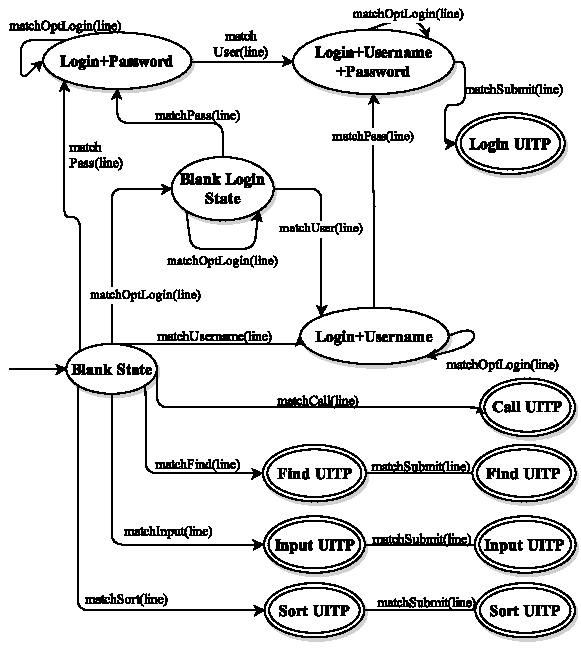
\includegraphics[width=\textwidth]{Global_State_Machine.pdf}
\caption{The inferrer's reasoning algorithm, expressed in a finite state machine.}
\label{fig:inferrer}
\end{figure}

For simplicity's sake, only the valid paths are shown in the figure (Fig. \ref{fig:inferrer}). All patterns except \textit{Login} can be valid even in the absence of a form submit action; this is done to account for dynamic submission via Javascript. In the case of the Login pattern, there can only be one password and one username or email record; this is done to distinguish login forms from register forms and password/email change forms.\\

The previous figure (Fig. \ref{fig:inferrer}) does not account for the \textit{Menu} and \textit{Master Detail} patterns; as mentioned before, these patterns are identified through HTML analysis and passed directly from the \textit{WebsiteExplorer} to the \textit{PatternInferrer} to write. This grammar only deals with the patterns identifiable through the execution trace file.\\

After the file is processed, an XMI file is produced containing all the pattern occurrences found, and the values assigned to each variable, as per Formula \ref{eq:ui_}. As mentioned before, the checks to perform within each test strategy and any preconditions must be specified by the tester later on in the PARADIGM-ME tool.\\

An example of a execution trace file extract from which a Login pattern can be inferred can be seen in Table \ref{tab:fullpattern}, and full example of a PARADIGM file (with inputs being  the contents of Table \ref{tab:fullexec} and Listing \ref{lst:full_exec_proc}) can be seen on Listing \ref{lst:full_pattern}.

\begin{table}[!htb]
\resizebox{0.9\textwidth}{!}{
\begin{tabular}{|c|c|c|c|}
\hline
\textbf{Action} & \textbf{Target} & \textbf{Value} & \textbf{Processing Return} \\ \hline
 & //a[@class=active &	 &  \\
clickAndWait & and @href=\ldots & EMPTY & clickLogin pageChange\\
&  and contains(text(),'Login')] & &  \\\hline
 & //input[@id=email & &  \\
type&  and @name=email & login@en.pt  & typeEmail\\
&  and @type=text] & & \\\hline
 & //input[@id=password  & &  \\
type& and @type=password & pass & typePassword\\
& and @name=password] & & \\\hline
 & //input[@id=save\_login &  &   \\
click& and @name=save\_login & EMPTY & clickLogin\\
&  and @type=checkbox] & & \\\hline
 & //input[@class=btn\_small grey &  &  \\
clickAndWait& and @name=commit & EMPTY & clickSubmit pageChange \\
&  and @type=submit] & & \\\hline
\end{tabular}
}
\caption{Execution trace example from which a Login pattern can be inferred.}
\label{tab:fullpattern}
\end{table}

\subsubsection{PARADIGM files produced by PatternInferrer}
The final PARADIGM files produced contain instances of UI Test Patterns, that correspond to all of the patterns discovered during the exploration made by the WebsiteExplorer and contain blank test configurations meant for the tester to fill in. The files are XMI files which follow the PARADIGM DSL (see Section \ref{sec:dsl}).

Each pattern is stored in a $<$\textit{nodes}$>$ tag, which has the following attributes: \textit{type} (the type of pattern), \textit{name} (a unique string identifier), \textit{number} (a unique integer identifier), \textit{incomingLinks} (the incoming sequence connector) and \textit{outgoingLinks} (the outgoing sequence connector).

Each $<$\textit{nodes}$>$ tag has two types of children: $<$\textit{configurations}$>$ tags, which contain testing configurations, and $<$\textit{fields}$>$ tags, which identify web elements involved in the testing configurations. Configurations are defined by attributes, and the specification of the test (such as data to insert or element to choose) are defined in $<$\textit{fields}$>$ child nodes. Some of the attributes that a configuration may have are: \textit{validity} (whether the inserted data is supposed to be valid or not); \textit{check} (the type of check to apply to the result of the operation); \textit{result} (the number of results expected - for testing Find patterns); \textit{master} (identifies the master in a MasterDetail pattern); and \textit{mappingURL} (the URL in which the testing elements are).

A simplified example of a generated model can be seen in Listing \ref{lst:paradigm_model}, in the Appendix chapter (Section \ref{sec:appendix}), and the corresponding graphic model, generated via PARADIGM-ME, can be seen in Figure \ref{fig:pbgt-me}.

\begin{figure}[!htb]
\centering
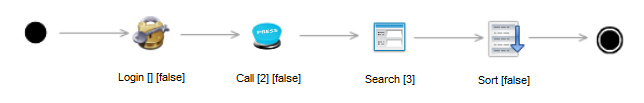
\includegraphics[width=\textwidth]{pbgt-me.png}
\caption{A simplified example of a generated model.}
\label{fig:pbgt-me}
\end{figure}

\section{Chapter Conclusions}
In this chapter we gave a brief overview of PGBT, explained in detail the previous and current tool, to better highlight their differences and explain their functioning. The previous tool requires user interaction to explore a Web application, analyzes the execution trace file, HTML source and URLs  of all pages visited, and infers patterns through a set of heuristic rules; the current tool is fully automatic, requires only the execution trace file, and infers patterns through syntactical analysis of a previously tokenized execution trace file.
